\chapter{Related Work}
\label{chap:related-work}

\section{Existing Evaluation Libraries and Observability Tooling}
\label{sec:existing_eval_libraries}

Alongside academic benchmarks, several practical libraries have emerged for evaluating LLM applications during development. These tools are useful because they move evaluation closer to the developer workflow: test cases can be rerun, prompts and models can be compared, and failures can be inspected more systematically than with ad hoc scripts. However, they also show that current tooling is still only partially suited to evaluating stateful, tool-using agents.

\subsection{OpenAI Evals}

OpenAI Evals is an open-source framework for evaluating LLMs and LLM systems \cite{openaiEvals}. It provides a general structure for defining datasets, running models on examples, and grading the resulting outputs. This is useful when developers want repeatable evaluation suites for comparing model versions or prompt changes. Evals can also use model-graded checks, where another LLM judges whether the output satisfies some rubric.

The limitation is that OpenAI Evals is still mainly organised around examples and graders. This works well for many single-turn tasks, but is less natural for agent evaluations where the important behaviour may be distributed across several turns, tool calls, and state changes. It can be extended with custom logic, but the framework does not provide a particularly direct scenario-level language for asserting, for example, that a user-facing output, a sequence of tool calls, and the resulting application state are all correct together.

\subsection{DeepEval and Ragas}

DeepEval and Ragas provide more application-oriented evaluation abstractions. DeepEval presents LLM evaluation in a unit-testing style and ships ready-made metrics, including G-Eval \cite{liu2023geval}, alongside measures for RAG, conversations, safety, and agentic behaviour \cite{deepevalDocs}. Its tool correctness metric evaluates whether expected tools were called, with options to consider input parameters and tool outputs \cite{deepevalDocs}.

\begin{figure}[htbp]
  \centering
  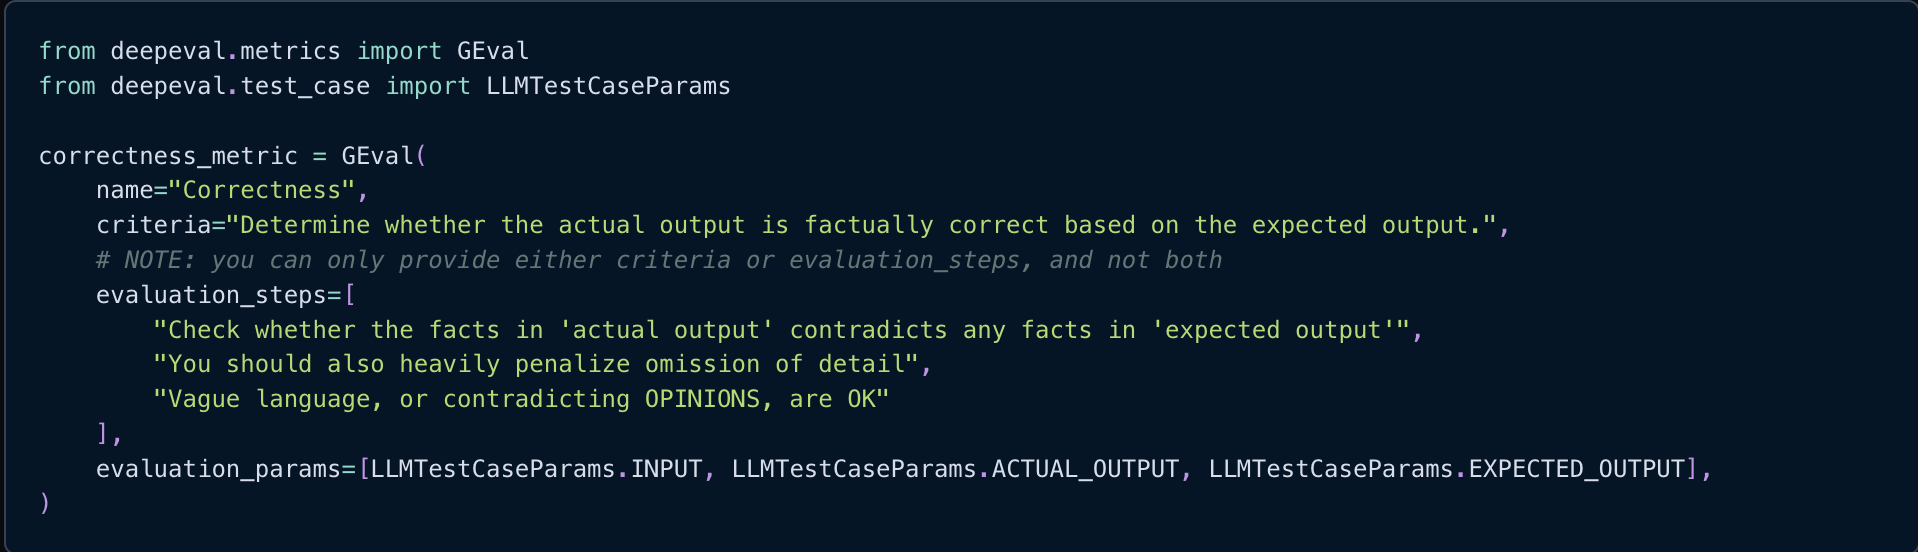
\includegraphics[width=0.8\textwidth]{figures/geval_instantiation_code_snippet.png}
  \caption{G-Eval prompt instantiation using the DeepEval library: evaluation criteria and chain-of-thought instructions are composed into a judge prompt for scoring model outputs \cite{liu2023geval,deepevalDocs}.}
  \label{fig:geval-prompt}
\end{figure}

Ragas was originally designed for RAG evaluation, decomposing quality into dimensions such as faithfulness, answer relevance, context precision, and context recall \cite{es2023ragas,ragasDocs}. More recent versions also include agent metrics such as tool call accuracy, tool call F1, and agent goal accuracy \cite{ragasDocs}. Agent goal accuracy is a binary multi-turn metric: an evaluator LLM reads the full interaction trace, infers the outcome the agent reached, and judges whether it matches the user's goal, either against a provided reference outcome or by inferring the goal from the conversation \cite{ragasDocs}.

These libraries are valuable because they recognise that LLM systems should not only be judged by final-answer quality. However, their tool checks are still relatively metric-oriented. They are useful for comparing expected and actual tool calls, but they are less ergonomic when a developer wants to specify precise properties of a tool argument or a structured output. For example, checking that a particular tool argument contains the substring \texttt{urgent}, or that a nested structured output field satisfies a domain-specific predicate, is not usually a first-class assertion. It generally requires custom code, a custom metric, or reshaping the output into the format expected by the evaluator. This makes simple behavioural expectations feel heavier than ordinary software tests.

\subsection{Promptfoo}

Promptfoo is an open-source tool for evaluating and red-teaming LLM applications using declarative test cases \cite{promptfooDocs}. It supports prompt and model comparison, assertions, CI/CD workflows, caching, and multiple providers. It also includes deterministic assertions such as equality, substring containment, regex matching, JSON validation, and custom JavaScript or Python assertions \cite{promptfooDocs}. This makes it closer to traditional test-driven development than many purely metric-based evaluation frameworks.

Promptfoo is therefore one of the more practical tools for developer-led LLM testing. However, its main abstraction is still the prompt/application test case and its assertions. More complex agent checks, especially those involving multi-turn traces, tool-call arguments, structured outputs, and stateful side effects, can become awkward unless the developer writes custom assertion logic. It provides a useful assertion vocabulary, but it is less focused on representing a full agent scenario as a single object with output checks, tool checks, and state checks expressed together.

\subsection{Observability-Focused Tools}

A related group of tools focuses on observability rather than evaluation alone. LangSmith provides tracing, evaluation, prompt testing, feedback collection, and production monitoring for LLM applications \cite{langsmithDocs}. Langfuse similarly provides open-source application tracing, prompt management, evaluation, user feedback, and monitoring for LLM systems \cite{langfuseDocs}.

\begin{figure}[htbp]
  \centering
  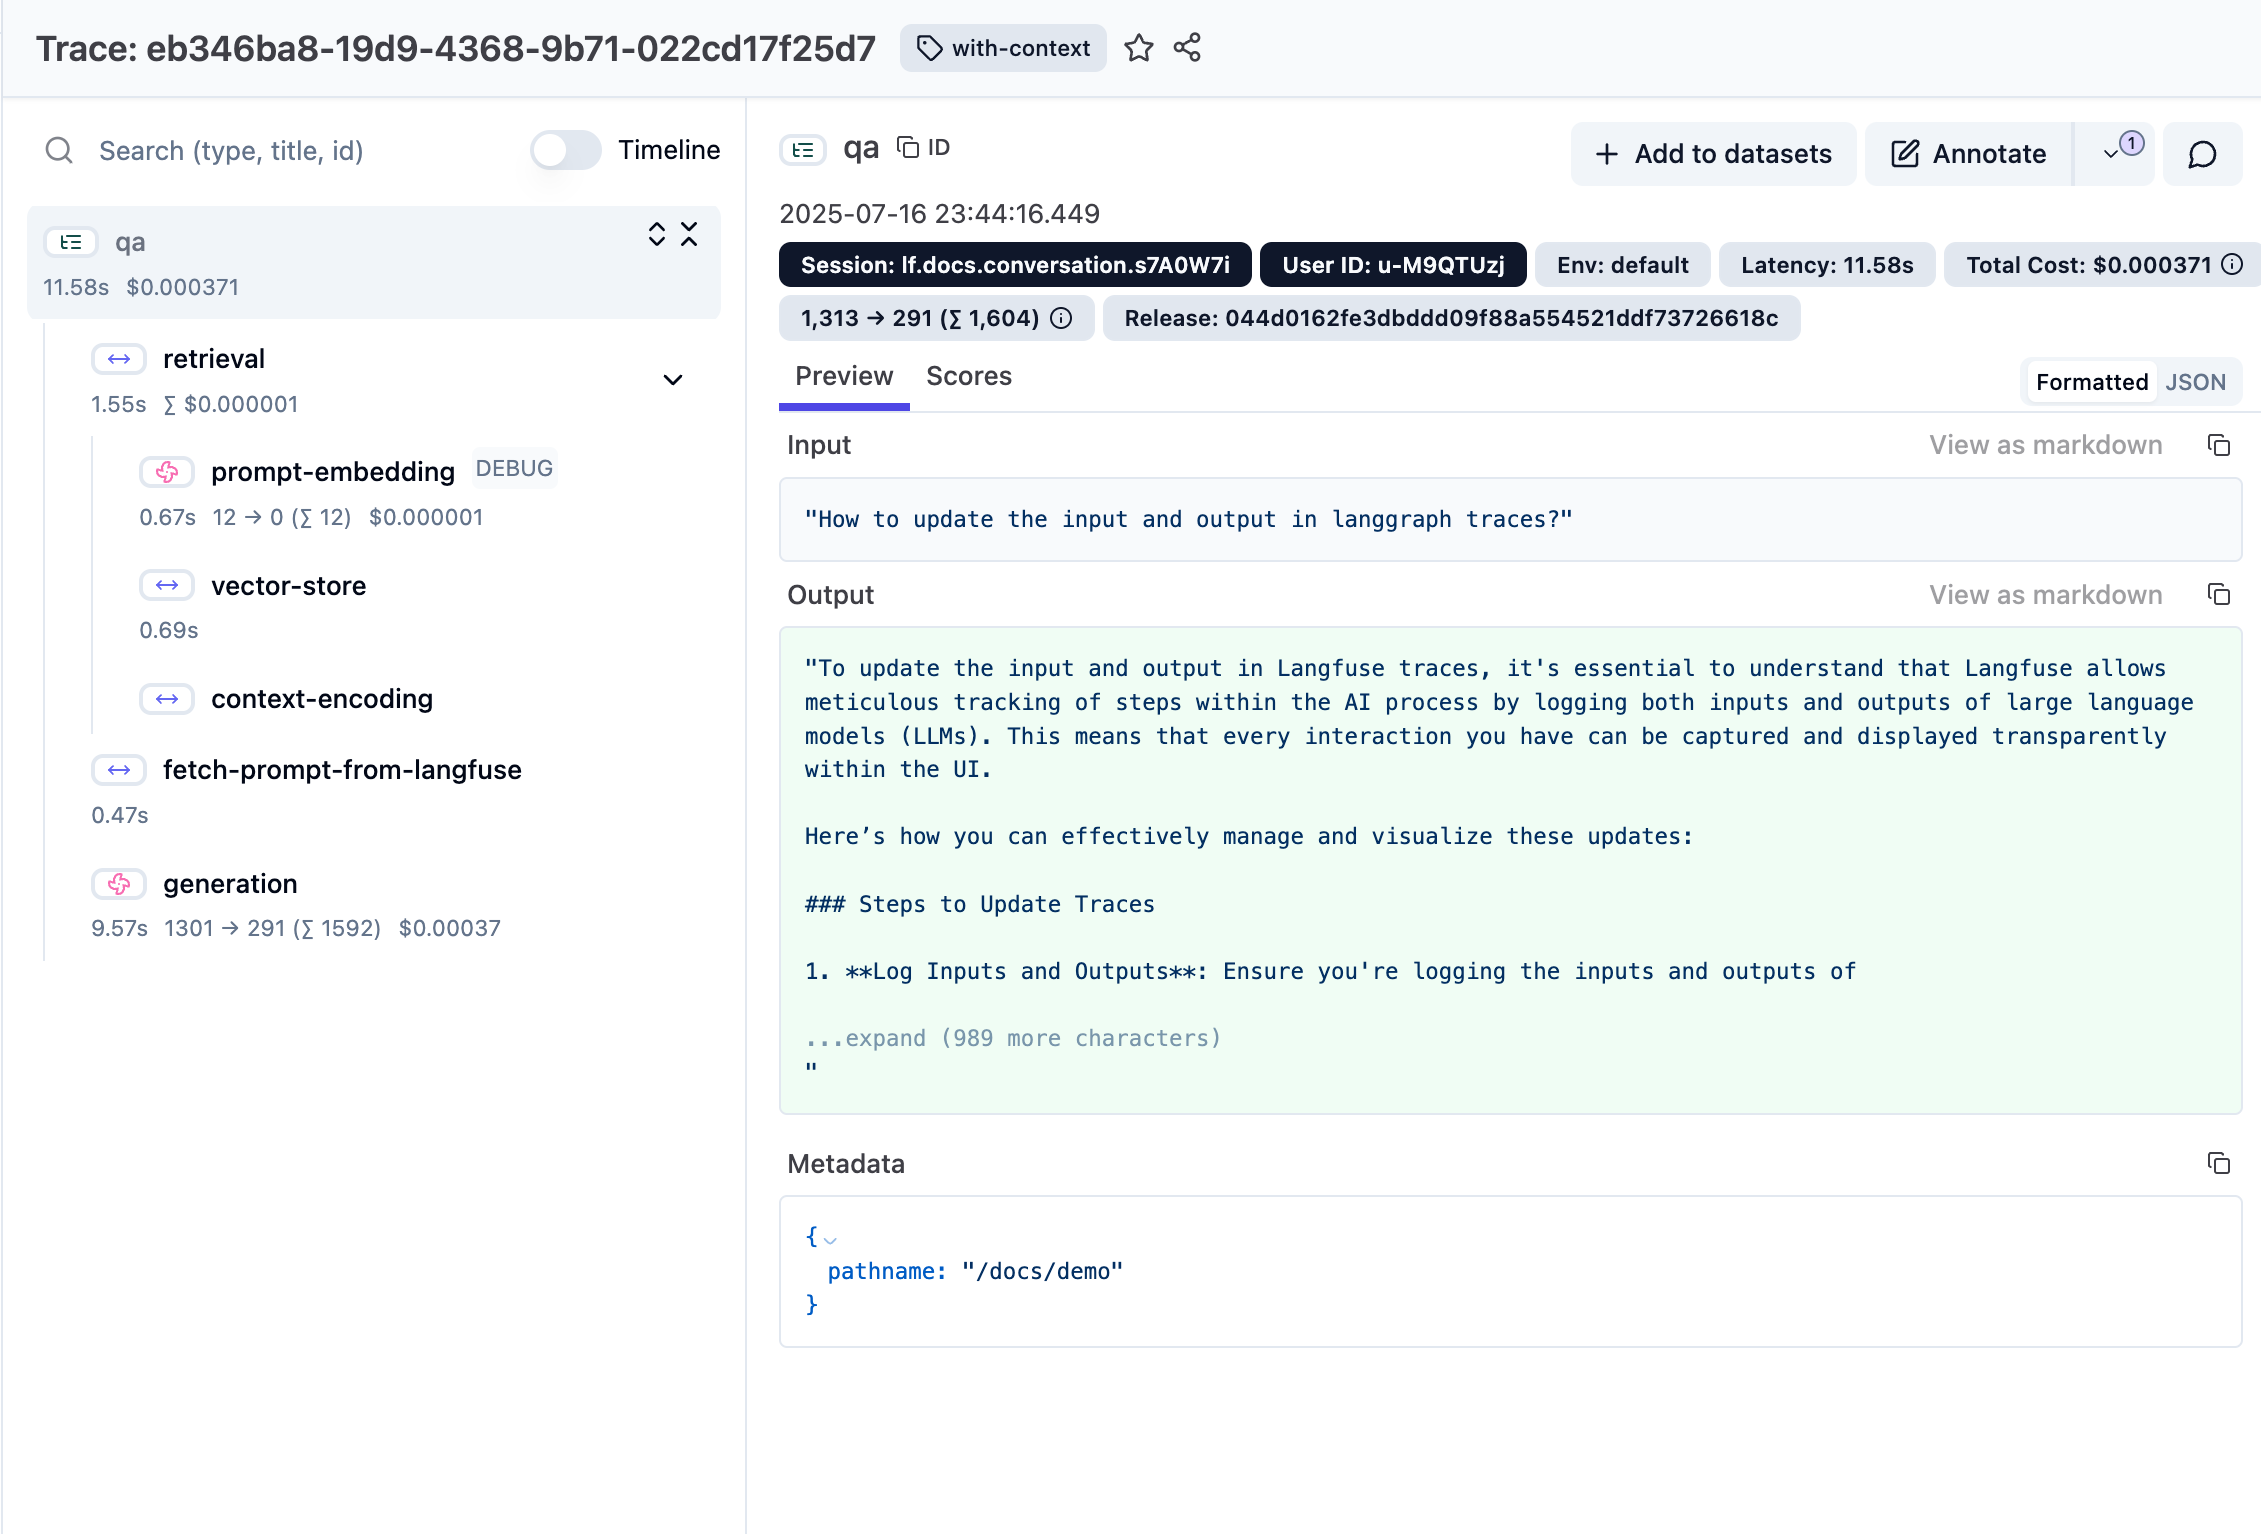
\includegraphics[width=0.88\textwidth]{figures/langfuse_example_trace.png}
  \caption{Example Langfuse trace for a RAG-style QA request: nested observations record retrieval (embedding and vector-store lookup), prompt retrieval, and final generation, with per-step latency, token usage, inputs, outputs, and cost \cite{langfuseDocs}.}
  \label{fig:langfuse-trace}
\end{figure}

These tools are important because agent failures are often hard to understand without seeing the full execution trace: the prompts, model responses, tool calls, tool outputs, intermediate steps, latency, and cost.

Observability tools are therefore highly complementary to evaluation libraries. They help developers inspect what happened during a run. However, observability does not by itself define what should have happened. A trace viewer can show that a tool was called, but the developer still needs a concise way to specify that the tool should only have been called after another condition, that its arguments should satisfy particular properties, that the final output should mention a required concept, and that the external state should end in a valid configuration.

\subsection{Gaps in Existing Libraries}

Existing libraries cover many important parts of the evaluation workflow, but they leave a gap for scenario-driven agent testing. Some tools are strong at scoring final outputs. Others provide RAG or tool-use metrics. Others provide trace observability and production monitoring. What is still missing is a developer-friendly way to define a complete agent scenario and attach explicit checks over the different surfaces of behaviour.

In particular, current tooling does not make it easy enough to combine output assertions, tool-call assertions, and state assertions in one coherent test. A developer should be able to express checks such as: the final response contains a required phrase, a particular tool was called with an argument satisfying a property, a forbidden tool was not called, and the resulting state matches the intended outcome. These checks should be easy to read, easy to modify, and should produce useful diagnostic output explaining which part of the scenario failed.

This is especially important for LLM agents because failures are often not visible in the final response alone. An agent may answer politely while calling the wrong tool, using the wrong argument, skipping a required step, or leaving the system in an invalid state. Conversely, a generic score may indicate failure without showing whether the problem was in the output, the tool trajectory, or the state transition. The main gap is therefore not simply the absence of metrics, but the absence of concise scenario-style evaluation tooling that treats the full agent trace as the object being tested.

\section{Motivation for Agent-Spec-Kit}
\label{sec:agent-spec-kit-motivation}

Chapter~\ref{chap:background} argues that agent evaluation must cover traces, tools, state, and repeated runs, not only final answers. Benchmarks such as AppWorld, $\tau$-bench, and ToolSandbox show why \cite{trivedi2024appworld,yao2024taubench,lu2024toolsandbox}; software-testing work shows how to find, simplify, and preserve failures \cite{claessen2000quickcheck,zeller2002simplifying,yu2023gptfuzzer,yao2023fuzzllm}. The preceding section shows that existing libraries and observability tools still do not make it easy to express those checks together in one scenario.

The remaining gap is developer-facing: a way to specify, run, inspect, and rerun behavioural tests for a custom agent without adopting a fixed benchmark or writing large amounts of custom glue code. Agent-Spec-Kit targets that gap. It treats an agent episode as a testable scenario with explicit checks over the final output, tool calls, and environment state, and it supports workflows such as repeated trials, generative variation, failure shrinking, and regression extraction described in the methodology chapter.
